 \section{Description and Analysis of the Domain}
 Today,people live comfortable life,because of the favourable progress of technology.A lot of things that people had to do by themselves even few years ago become the work of machines today.It is essential to understand that during the next few decades or maybe sooner, the notion of work and whether it is handled by a human will be replaced by software,instead of using the ancient approach of doing everything individually.However someone believes that this progress make people lazy,saying people rely on machines too much,actually it makes human beings more active both physically and mentally,machines or high technology help people to complete tasks more quickly.
 
 Time and money are those two key points which people are in rush for continuously and their right management are a priority nowadays.Here is the point of using technologies for repetitive operations, in such a way,mistakes are reduced or eliminated, and the time it takes to complete the task is greatly reduced.Diving deeper into the subject,an application which will manage the money and simultaneous will save the time by doing the action quickly is exactly what society needs.
 
 Spending Tracker is a mobile application that comes with a solution for existing problem in the society, of managing right the budget and saving the time on doing that.Scheduling periodically the budget reviews and stick to a strict plan to bring the financial health of the family in line with the goals.So,such an application brings a lot of benefits to its users as:
 \begin{itemize}
 	\item Gives control over user's money;
 	\item Accelerates financial goals;
 	\item Helps in organizing spending and savings;
 	\item Enables saving for expected and unexpected costs;
 	\item Enables to produce extra money
 	\item Aligns priorities;
 	\item Builds new habits;
 \end{itemize}
 
\subsection{The workflow of the system}
In order to be able to access the Spending Tracker application,a user should first of all install it on an Android platform, which is made simply by pressing install button in Android Play Store.Once the application is opened,a Welcome screen is displayed.The Welcome screen serves as an introduction point for users such as there, in a pager are described the basic futures of the application, in such a way user is getting ready to use the application.Then by pressing start button, the main view is opened which contains the basic information about the expenditures of default today date.If to expend the spinner from the left top corner then can be observed the lists of all the features which the application offer to use.

The application itself offers some statistics about the amounts spend on different categories of stuff in different stores.User can see on what product he spends most and receive some advices as an alert if it's case to save on something.The next action which can be performed is scanning of receipts which is made by pressing the bottom right corner plus button which opens another view with all necessary information about scanning the receipt.It's necessary to press another bottom button "TAKE A PHOTO OF YOUR RECEIPT" which starts the phone video camera and capture a photo for forward use. After capturing when clicking "OK" button for storing data, an alerting windows may appear in case one product is cheaper in the current store than in others.Another moment that gives an additional credit to the discussed product is the fact that the user can choose the period for showing the total amount spend,it's possible to see amount for today, for the week or an entire month.Assuming that project is in its early development stage,a lot of useful functionalities are going to be added further.

\subsection{Similar products on the market}
The idea of creating the discussed application came first of all from the society needs.Often are tackled subjects like saving for the future, paying off debt and protecting what people have got and everyone is complaining about lack of knowledge in how to do all of enumerated actions.

Spending is highly individual stuff.Beyond the golden rule—spend less than you earn—it’s hard to be prescriptive because expenditures are the result of so many individual decisions, many of which feel not significant as people make them.So,in order to solve the frequently asked questions by the people "to spend on this" or "don't spend on that",today exists plenty of mobile and web applications which try somehow to track people's outflows.

 Assuming that, in order to create a good software, it is necessary to make a market research and find similar solutions to the problems that are being solved by that software, making a connection between the system to be developed and the missing features in the existing similar applications.The Receipt Scanner application was inspired from another existing ones but with lack of the basic functionality - automated scanner of receipt through the phone video camera, and storing all the content of receipt in a digital text which allows to perform a lot of actions on it forward.According a Forbes research \cite{Forbes} almost all of existing similar applications require a manual input of the expenditures,which is somehow inconvenient and requires more time to do.

If to analyse some actual examples of such applications,can be observed that all of them require a manual input,besides this they have a lot of other nice functionalities which can be used as well for the receipt scanner further.

\textbf{Dollarbird} - Add past or future income and expenses to a calendar that calculates the impact on people balance, as well as spending by category. The basic features are:
\begin{itemize}
	\item Price: Free
	\item Links to accounts: No
	\item Manual input: Yes
	\item Available on: iOS, Android
\end{itemize}
\begin{figure}[H]
	\centering
	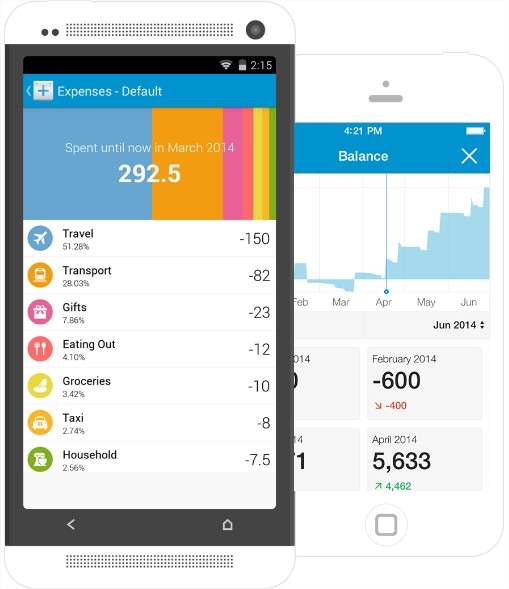
\includegraphics[width=12cm]{Chapter1/Dollarbird.jpg}
	\caption{Dollarbird Application, \cite{Dollarbird}}
	\label{fig:Dollarbird}
\end{figure}

\textbf{Goodbudget} - Recreates envelope budgeting of yesteryear for the digital world. Set a budget for each category and spend from that designated category. When the money run out stop spending.Bellow are represent some basic features:
\begin{itemize}
	\item Price: Free; \$45/year for unlimited categories, five years of history, to sync up to five devices
	\item Links to accounts: No
	\item Manual input: Yes
	\item Available on: iOS, Android
\end{itemize}
\begin{figure}[H]
	\centering
	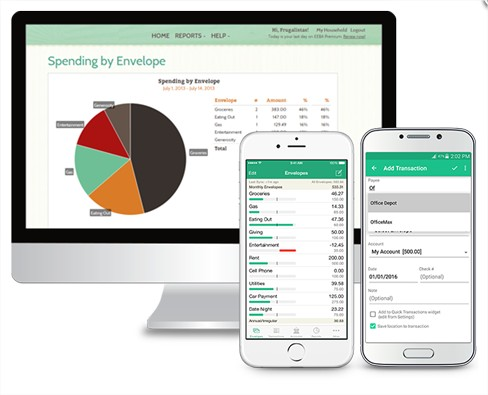
\includegraphics[width=12cm]{Chapter1/Goodbudget.jpg}
	\caption{Goodbudget application, \cite{Goodbudget}}
	\label{fig:Goodbudget}
\end{figure}

\textbf{mvelopes} -  Like GoodBudeget, mvelopes is a spin on classic envelope budgeting but with account integration. Some basic features are enumerated bellow: 
\begin{itemize}
	\item Price: Free; \$95/year to link unlimited accounts and to create more than 25 envelopes, as well as for a debt management tool
	\item Links to accounts: Yes
	\item Manual input: Yes
	\item Available on: iOS, Android
\end{itemize}
\begin{figure}[H]
	\centering
	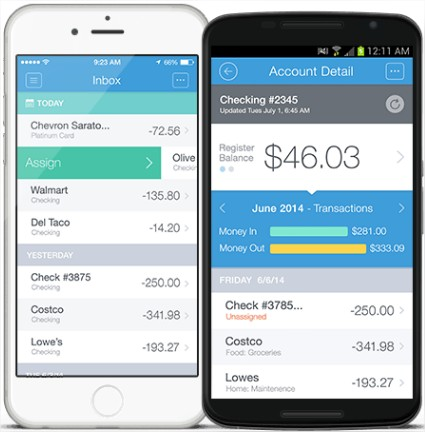
\includegraphics[width=12cm]{Chapter1/Mvelopes.jpg}
	\caption{Mvelopes Application, \cite{Mvelopes}}
	\label{fig:Goodbudget}
\end{figure}
So existing applications on market can serve as a prototype of the Receipt Scanner, with some improvement in that area of automating the process of manual input.

\subsection{The development environment}
Building an Android application comes down to two major skills or languages: Java and Android. Java is the language used in Android, but the Android part surround learning XML for the design of the application, learning the concepts of Android, and using the concepts programmatically with Java.The Mobile Vision Text API gives a powerful and reliable Optical Character Recognition (OCR) capability that works with most Android devices,that's why this is exactly technology which is used for recognizing easily all the text from a receipt.

When writing an Android application,there are some primary points which need to be taken in consideration:
\begin{itemize}
	\item Describing and modelling the application's domain which represents the universe of the application is the key point before starting.In this case, the domain represents an application that would allow scanning the receipts and will return a budget report,weekly,monthly or even daily.At this point need to be established what's in it,how many views and actions contains the application and what is the relation between them.This is like modelling a database structure to keep the entities and their relationship.
	\item Specifying what can happen in this domain is another key point, it is necessary to identify all the possible scenarios or actions that the elements of the domain can participate in.
	\item Choosing the right IDE(Integrated Development Environment) is not less important point.The most common IDE for Android development and that used for the current project is named Android Studio,it comes direct from the Google itself.It gives the main UI when code is entered,it highlights things which are wrong,offers suggestions and lets running and testing creations conveniently.It creates files, provides basic layouts and generally it saves a lot of time and effort.
\end{itemize}
\subsubsection{Back-end implementation: Java for Android}
For implementing the idea of Spending Tracker, Java for Android language was chosen. Such as the application from the start point was designed to be a mobile application,then there was not a better choice than to use Java,it's really the only option for native applications.It is one from the most popular programming languages,namely for its important core features as are: 
\begin{itemize}
	\item easy to learn and understand;
	\item designed to be a platform-independent and secure,using virtual machines;
	\item it's object oriented.
\end{itemize} 
Android relies intensely on these Java fundamentals. The Android SDK includes many standard Java libraries as well as special Android libraries, as is Mobile Vision Text API for Android, the basic library used in developing Spending Tracker.

Spending Tracker application is based generally on OCR (Optical Character Recognition) used with Mobile Text API for Android. OCR gives a computer the ability to read text that appear in an image. The Mobile Vision Text API gives Android developers a powerful nd reliable OCR capability that works with most Android devices and won't increase the size of the application.\cite{Codelabs}

Text recognition is the process of detecting text in images, video streams and recognizing the text contained in.When it is detected,than the recognizer determines the actual text in each block and segments into lines or words.The Text API recognize text in any Latin based language.
\cite{Text Recognition API}

In software applications, it is mostly required to store user’s and application data locally, so that was stored for Spending Tracker as well.\textbf{Realm} is one of the way of storing data provided by Android SDK. Realm is is a mobile database and a replacement for SQLite.Realm store data in a universal, table-based format by a C++ core. This is what allows Realm to allow data access from multiple languages as well as a range of ad hoc queries.
Some key points for understanding better Realm are enumerated bellow:\cite{Realm}
\begin{itemize}
	\item faster than SQLite (up to 10x speed up over raw SQLite for normal operations)
	\item easy to use
	\item object conversion handled for user
	\item convenient for creating and storing data on the fly
	\item very responsive team
\end{itemize}

\subsubsection{ Model-View-Controller architecture}
This chapter can be started with the best expression about MVC architectural patterns: "The only way to make the deadline—the only way to go fast—is to keep the code as clean as possible at all times.",said by \textit{Robert C. Martin, Clean Code: A Handbook of Agile Software Craftsmanship}\cite{MVC in Android}.

MVC is an architectural pattern which means \textbf{Model,View,Controller} and its aim is to provide kind of a “template” for organization of software system.The idea of MVC is that of dividing the software into three independent components:
\begin{itemize}
	\item The component that stores system’s state (whether this state persistent or not). This component is referred to as \textbf{Model}.
	\item The component that handles input-output from/to the client (the client might be a human user, but it doesn’t have to). This component is referred to as \textbf{View}.
	\item The component that represents the logical functionality of the system, holds system’s “business rules”. This component is referred to as \textbf{Controller/Presenter}.
\end{itemize}
Bellow are represented interaction diagrams for that two similar architectural patterns MVC and MVP,the differences are not such significant,but for Android development, MVP is more suitable and next will be explained why so.
\begin{figure}[H]
	\centering
	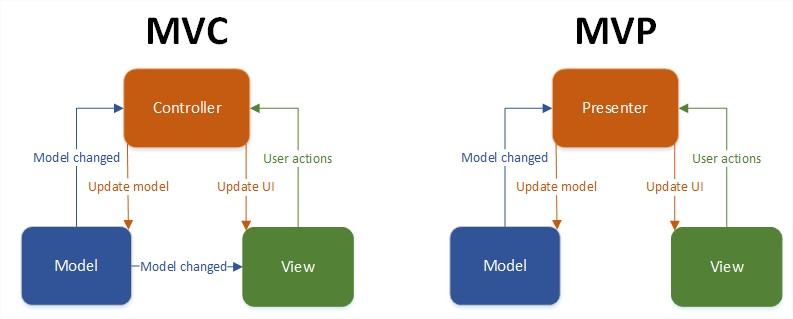
\includegraphics[width=12cm]{Chapter1/mvc-android.jpg}
	\caption{MVC pattern integration with Android, \cite{MVC}}
	\label{fig:MVC-Android}
\end{figure}

MVP was proved to be more suitable for Android development due to very tight coupling between Activities and Fragments (which are MVP presenters) and various parts of Android framework. The "Model" part is fine -  it is straightforward to implement a standalone model functionality in Android. The problems arise if to try to separate view and controller functionality.For example \textit{onCreate()} method,which is called by Android framework in response to framework’s internal state transitions (these transitions might be related to user’s actions in the app,  but the app never calls onCreate() directly). So can be created an impression that this method belongs to the “view” part of MVC because setContentView() is called along the way, but, in fact, setContentView() is a standard binding of a view performed by the controller.

In MVP, the view knows nothing about the model, and it is presenter’s job to fetch the up to date data from the model, understand whether the view should be updated and bind a new data to the view. In MVP, the logic contained in MVC view, is located in the presenter, which makes the views very “stupid” – their sole purpose becomes rendering data that was bound to them by the presenter.Finally, good MVP model tends to just manage application’s data state and notify presenters of any change, nothing more.

\subsubsection{Front-end implementation in Android}
Android front-end implementation could be defined in two ways:
\begin{itemize}
	\item \textbf{Declare UI elements in XML.} Android provides a straightforward XML vocabulary that corresponds to the View classes and subclasses, such as those for widgets and layouts.
	\item \textbf{Instantiate layout elements at runtime.}The application can create View and ViewGroup objects (and manipulate their properties) programmatically.
\end{itemize}
It is possible to use either or both of these methods for declaring and managing the application's UI.The advantage of declaring the UI in XML is that it enables to better separate the presentation of the application from the code that controls its behaviour.The UI descriptions are external to the application which means that application can be modified and adapted without modifying the source code and recompiling.Also, declaring the UI using XML makes it easier to visualize structure of UI,it's easier to debug problems.

In general, the XML vocabulary for declaring UI elements closely follows the structure and naming of the classes and methods, where element names correspond to class names and attribute names correspond to methods. \cite{Android XML} 
